\documentclass{beamer}
\usetheme{Madrid}
\usecolortheme{dolphin}
\usepackage{graphicx}
\usepackage{listings}
\usepackage{xcolor}
\usepackage{caption}

\definecolor{codegreen}{rgb}{0,0.6,0}
\definecolor{codegray}{rgb}{0.5,0.5,0.5}
\definecolor{codepurple}{rgb}{0.58,0,0.82}
\definecolor{backcolour}{rgb}{0.95,0.95,0.92}

\lstdefinestyle{mystyle}{
    backgroundcolor=\color{backcolour},   
    commentstyle=\color{codegreen},
    keywordstyle=\color{magenta},
    numberstyle=\tiny\color{codegray},
    stringstyle=\color{codepurple},
    basicstyle=\ttfamily\footnotesize,
    breakatwhitespace=false,         
    breaklines=true,                 
    captionpos=b,                    
    keepspaces=true,                 
    numbers=left,                    
    numbersep=5pt,                  
    showspaces=false,                
    showstringspaces=false,
    showtabs=false,                  
    tabsize=2
}

\lstset{style=mystyle}

\title{Interactive Drawing Tool}
\subtitle{A Java-based Drawing Application}
\author{AP Computer Science A Project}
\date{\today}

\begin{document}

\begin{frame}
\titlepage
\end{frame}

\begin{frame}{Demo}
\begin{center}
% \includegraphics[width=0.8\textwidth]{example-image} % Replace with actual screenshot

% \vspace{0.5cm}
% \textbf{Interactive Drawing Tool}\\
% A Java-based drawing application with layer support, similar to basic image editing software.

% \vspace{0.3cm}
% \textit{Features:} Drawing tools, layer management, shape manipulation, undo/redo, and file operations
\end{center}
\end{frame}

\begin{frame}{Project Overview}
\begin{itemize}
\item A Java Swing-based drawing application
\item Provides multiple drawing tools (line, rectangle, circle, text, free drawing)
\item Supports layer management for complex drawings
\item Includes selection and manipulation of shapes
\item Features undo/redo functionality
\item Allows saving and loading drawings
\item Implements zoom and pan capabilities
\end{itemize}
\end{frame}

\begin{frame}{Design Principles}
\begin{columns}
\column{0.5\textwidth}
\textbf{Object-Oriented Design}
\begin{itemize}
\item Inheritance hierarchy for shapes
\item Encapsulation of functionality
\item Polymorphism for drawing operations
\end{itemize}

\column{0.5\textwidth}
\textbf{Design Patterns}
\begin{itemize}
\item Model-View-Controller pattern
\item Command pattern for undo/redo
\item Observer pattern for UI updates
\item Strategy pattern for drawing tools
\end{itemize}
\end{columns}

\vspace{0.5cm}
\begin{center}
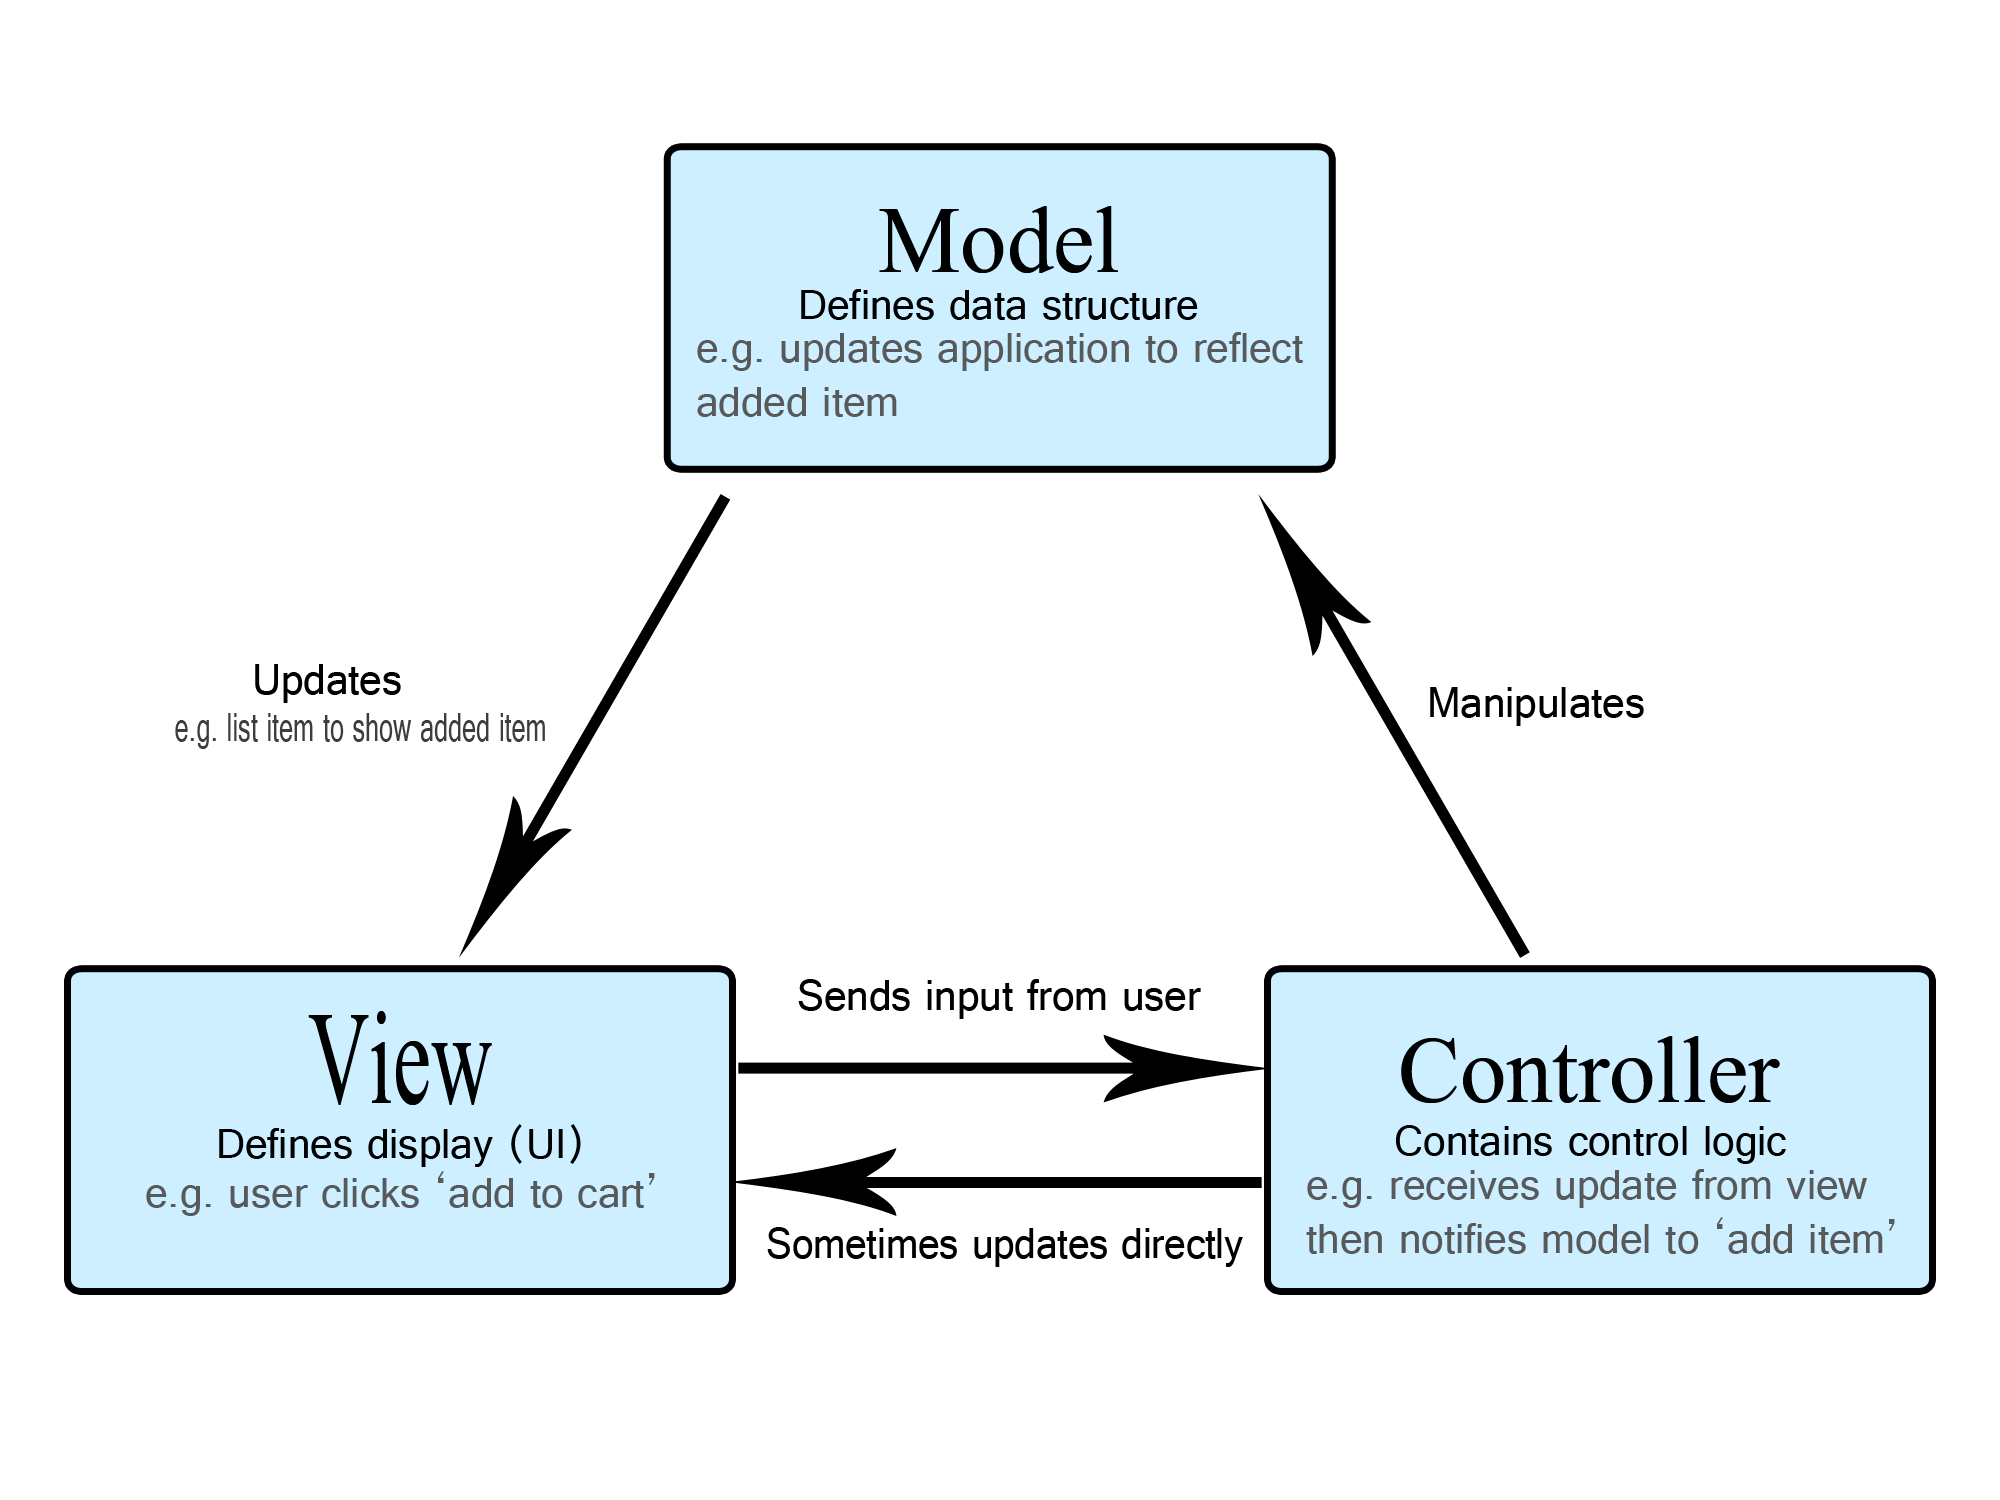
\includegraphics[width=0.6\textwidth]{images/model-view-controller-light-blue.png}
\captionof*{figure}{Model-View-Controller Pattern}
\end{center}
\end{frame}

\begin{frame}{Architecture Overview}
\begin{center}
\begin{tabular}{|l|l|}
\hline
\textbf{Component} & \textbf{Purpose} \\
\hline
DrawingApp & Main application window and UI \\
\hline
DrawingPanel & Canvas for drawing and interaction \\
\hline
Shape & Abstract base class for all shapes \\
\hline
Layer & Container for organizing shapes \\
\hline
LayerPanel & UI for managing layers \\
\hline
\end{tabular}
\end{center}
\end{frame}

\begin{frame}{Class Hierarchy}
\begin{center}
\begin{tabular}{c}
\texttt{Shape} (Abstract) \\
$\downarrow$ \\
\begin{tabular}{ccccc}
\texttt{Line} & \texttt{Rectangle} & \texttt{Circle} & \texttt{TextShape} & \texttt{FreeDrawing} \\
\end{tabular}
\end{tabular}
\end{center}

\vspace{0.5cm}
\begin{itemize}
\item \texttt{Shape}: Common properties and behaviors
\item Specific shape classes: Implement drawing logic
\item \texttt{Layer}: Contains and manages multiple shapes
\item \texttt{DrawingPanel}: Manages layers and user interaction
\end{itemize}
\end{frame}

\begin{frame}[fragile]{Core Component: Shape}
\begin{itemize}
\item Abstract base class for all drawable elements
\item Defines common properties:
  \begin{itemize}
  \item Coordinates (x1, y1, x2, y2)
  \item Color and stroke width
  \item Fill state (filled or outline)
  \item Selection state
  \end{itemize}
\item Provides methods for:
  \begin{itemize}
  \item Selection and manipulation
  \item Hit detection
  \item Drawing selection handles
  \end{itemize}
\end{itemize}

\begin{verbatim}
public abstract class Shape implements Serializable {
    protected Color color;
    protected int x1, y1, x2, y2;
    protected boolean filled;
    protected boolean selected;
    
    public abstract void draw(Graphics g);
    public boolean containsPoint(int x, int y) { ... }
}
\end{verbatim}
\end{frame}

\begin{frame}[fragile]{Core Component: Layer}
\begin{itemize}
\item Container for organizing shapes
\item Manages visibility and z-order
\item Provides shape selection functionality
\item Enables layer-specific operations
\end{itemize}

\begin{verbatim}
public class Layer implements Serializable {
    private String name;
    private ArrayList<Shape> shapes;
    private boolean visible;
    private boolean selected;
    
    public void draw(Graphics g) {
        if (visible) {
            for (Shape shape : shapes) {
                shape.draw(g);
            }
        }
    }
    
    public Shape getShapeAt(int x, int y) { ... }
}
\end{verbatim}
\end{frame}

\begin{frame}[fragile]{Core Component: DrawingPanel}
\begin{itemize}
\item Central canvas where drawing happens
\item Manages mouse and keyboard interactions
\item Creates appropriate shapes based on selected tool
\item Implements undo/redo functionality
\item Handles selection, moving, and resizing
\item Provides zoom and pan capabilities
\end{itemize}

\begin{verbatim}
public class DrawingPanel extends JPanel {
    private ArrayList<Layer> layers;
    private Layer currentLayer;
    private Stack<ArrayList<Layer>> undoStack;
    private Stack<ArrayList<Layer>> redoStack;
    private String currentShape;
    private Shape currentDrawing;
    // Mouse listeners, keyboard listeners, etc.
}
\end{verbatim}
\end{frame}

\begin{frame}[fragile]{Core Component: DrawingApp}
\begin{itemize}
\item Main application window
\item Creates all UI components:
  \begin{itemize}
  \item Menus and toolbars
  \item Drawing panel (canvas)
  \item Properties panel
  \item Layer panel
  \end{itemize}
\item Handles file operations
\item Connects user actions to drawing functionality
\end{itemize}

\begin{verbatim}
public class DrawingApp extends JFrame {
    private DrawingPanel drawingPanel;
    private JTextField textField;
    private JMenuBar menuBar;
    private JToolBar toolBar;
    private JToolBar propertiesBar;
    // UI creation methods, event handlers, etc.
}
\end{verbatim}
\end{frame}

\begin{frame}{Drawing Process}
\begin{enumerate}
\item User selects a drawing tool (e.g., Rectangle)
\item User presses mouse button on canvas
  \begin{itemize}
  \item \texttt{DrawingPanel} creates new shape instance
  \item Initial coordinates are set
  \end{itemize}
\item User drags mouse
  \begin{itemize}
  \item Shape's end coordinates are updated
  \item Canvas is repainted to show the shape being drawn
  \end{itemize}
\item User releases mouse button
  \begin{itemize}
  \item Shape is finalized and added to current layer
  \item Current state is saved for undo functionality
  \end{itemize}
\end{enumerate}
\end{frame}

\begin{frame}{Selection and Manipulation}
\begin{columns}
\column{0.5\textwidth}
\textbf{Selection Process}
\begin{enumerate}
\item User clicks on canvas
\item \texttt{DrawingPanel} checks all shapes from top to bottom
\item First shape containing the click point is selected
\item Selection handles are displayed
\end{enumerate}

\column{0.5\textwidth}
\textbf{Manipulation}
\begin{itemize}
\item \textbf{Moving:} Drag selected shape
\item \textbf{Resizing:} Drag selection handles
\item \textbf{Deleting:} Press Delete key
\item \textbf{Reordering:} Layer panel controls
\end{itemize}
\end{columns}
\end{frame}

\begin{frame}{Layer Management}
\begin{itemize}
\item Layers organize shapes in z-order
\item \texttt{LayerPanel} provides UI for:
  \begin{itemize}
  \item Creating new layers
  \item Deleting layers
  \item Changing visibility
  \item Reordering layers
  \end{itemize}
\item Drawing process:
  \begin{enumerate}
  \item \texttt{DrawingPanel.paintComponent()} is called
  \item Each visible layer is drawn in order (bottom to top)
  \item Each layer draws its shapes in order
  \end{enumerate}
\end{itemize}
\end{frame}

\begin{frame}{Undo/Redo Implementation}
\begin{itemize}
\item Uses command pattern with state snapshots
\item Each significant action:
  \begin{enumerate}
  \item Creates a deep copy of all layers
  \item Pushes copy to undo stack
  \item Clears redo stack
  \end{enumerate}
\item Undo operation:
  \begin{enumerate}
  \item Pops state from undo stack
  \item Pushes current state to redo stack
  \item Restores popped state
  \end{enumerate}
\item Redo operation: Reverses the undo process
\end{itemize}
\end{frame}

\begin{frame}{File Operations}
\begin{itemize}
\item \textbf{Saving Drawings}
  \begin{itemize}
  \item Renders all visible layers to a BufferedImage
  \item Saves image as PNG file
  \end{itemize}
\item \textbf{Opening Images}
  \begin{itemize}
  \item Loads PNG image into BufferedImage
  \item Creates new ImageShape containing the image
  \item Adds shape to current layer
  \end{itemize}
\item Uses Java's ImageIO library for file operations
\end{itemize}
\end{frame}

\begin{frame}{Special Features}
\begin{columns}
\column{0.5\textwidth}
\textbf{Zoom and Pan}
\begin{itemize}
\item Zoom with mouse wheel or keyboard
\item Pan with middle mouse button
\item Coordinate transformation between screen and canvas
\end{itemize}

\column{0.5\textwidth}
\textbf{Splash Screen}
\begin{itemize}
\item Professional loading screen
\item Fade-in and fade-out animations
\item Progress bar simulation
\end{itemize}
\end{columns}

\vspace{0.5cm}
\textbf{Font Selection}
\begin{itemize}
\item Custom JFontChooser dialog
\item Preview of selected font
\item Font family, style, and size options
\end{itemize}
\end{frame}

\begin{frame}[fragile]{Code Example: Creating a Shape}
\begin{verbatim}
// In DrawingPanel.mousePressed()
switch (currentShape) {
    case "Circle":
        currentDrawing = new Circle(currentColor, 
                                   canvasX, canvasY, 
                                   canvasX, canvasY, 
                                   filled);
        break;
    case "Rectangle":
        currentDrawing = new Rectangle(currentColor, 
                                      canvasX, canvasY, 
                                      canvasX, canvasY, 
                                      filled);
        break;
    case "Line":
        currentDrawing = new Line(currentColor, 
                                 canvasX, canvasY, 
                                 canvasX, canvasY, 
                                 filled);
        break;
    // Other shape types...
}
\end{verbatim}
\end{frame}

\begin{frame}[fragile]{Code Example: Drawing a Shape}
\begin{verbatim}
// In Rectangle.java
public void draw(Graphics g) {
    Graphics2D g2d = (Graphics2D) g;
    
    // Save original stroke
    Stroke originalStroke = g2d.getStroke();
    
    // Set stroke width
    g2d.setStroke(new BasicStroke(strokeWidth));
    
    // Set the color
    g2d.setColor(color);
    
    // Calculate actual rectangle coordinates
    int x = Math.min(x1, x2);
    int y = Math.min(y1, y2);
    int width = Math.abs(x2 - x1);
    int height = Math.abs(y2 - y1);
    
    // Draw filled or outline rectangle
    if (filled) {
        g2d.fillRect(x, y, width, height);
    } else {
        g2d.drawRect(x, y, width, height);
    }
    
    // Restore original stroke
    g2d.setStroke(originalStroke);
    
    // Draw selection handles if selected
    drawSelectionHandles(g);
}
\end{verbatim}
\end{frame}

\begin{frame}{Future Enhancements}
\begin{itemize}
\item \textbf{Additional Shape Types}
  \begin{itemize}
  \item Polygon, Star, Arrow, etc.
  \end{itemize}
\item \textbf{Enhanced Text Editing}
  \begin{itemize}
  \item In-place text editing
  \item Rich text formatting
  \end{itemize}
\item \textbf{Advanced Layer Features}
  \begin{itemize}
  \item Layer groups
  \item Layer blend modes
  \end{itemize}
\item \textbf{Selection Improvements}
  \begin{itemize}
  \item Multiple selection
  \item Grouping shapes
  \end{itemize}
\item \textbf{File Format Support}
  \begin{itemize}
  \item Native format to preserve layers and editability
  \item Export to SVG, PDF, etc.
  \end{itemize}
\end{itemize}
\end{frame}

\begin{frame}{}
  \begin{center}
    \large{\textbf{Thank You!}}
    
    \normalsize{Questions?}
  \end{center}
\end{frame}

\end{document} 